\section{Introduction}

\emph{myproof} est un logiciel de profiling, à la manière de \emph{gprof}\footnote{GNU gprof: \url{http://www.cs.utah.edu/dept/old/texinfo/as/gprof_toc.html}}, regroupant toutes les étapes nécessaire à l'instrumentation et à la mesure d'une application cible. Il se différencie, tout de même, de ce dernier en apportant une interface modulable. En effet, il devient possible avec \emph{myproof} d'integrer aisément, par exemple, sa propre ``pass''\footnote{une pass gcc} ou encore un nouveau ``pragma''\footnote{\#pragma directive}. Pour cela, \emph{myproof} fournit des structures de données complètes comme ``les fonctions'', ``les blocs de base'', ``les boucles'' mais aussi ``les chemins'' entre blocs de base.

\subsection{Hierarchie des fonctionnalités principales}

Nous présentons, en figure \ref{fig:hierarchy}, les fonctionnalités principales de notre logiciel de profiling. En partant de la racine du projet, nous avons 3 sous-noeuds qui sont respectivement ``gcc plugin'', ``profiler'' et ``report''. ``gcc plugin'' est le repertoire contenant le plugin. Il permet de charger à chaud les fonctionnalités de ``myproof'' durant la phase de compilation de gcc. ``profiler'' contient l'outil de profiling. ``report'' est le repertoire contenant ce jolie rapport. Nous verrons plus en détail, par la suite, les fonctionnalités de ``gcc plugin''.

\begin{figure}[here]
  \centering
  \begin{dot2tex}[neato]
    digraph G
    {
      node [fixedsize=true, width=0.4, style="fill=green!20"];
      "myproof" -> {"gcc plugin" "profiler" "report"};
      "gcc plugin" -> {"init" "passes" "pragmas" "summary" "error" "end" "measure"};
      "myproof" [style="fill=orange!80"];
      "gcc plugin" [style="fill=orange!40"];
    }
  \end{dot2tex}
  \caption{Hierarchy of main features}
  \label{fig:hierarchy}
\end{figure}

      % "passes" -> {"function pass" "basicblock pass" "loop pass" "bb pass" "variable pass" "instrumente pass"};
      % "pragmas" -> {"instrumente pragma"};
      % "summary" -> {"all data structures std output" "static instrumentation output"};
      % "error" -> {"checks existing instrumented function"};
      % "end" -> {"remove all data structures"};

      % "profiler" -> "python script";


% \begin{figure}[here]
%   \centering
% \begin{dot2tex}[dot,tikz,codeonly,styleonly,options=-s -tmath]
%   digraph G {
%     d2tdocpreamble = "\usetikzlibrary{automata}";
%     d2tfigpreamble = "\tikzstyle{every state}= \
%     [draw=blue!50,very thick,fill=blue!20]";
%     node [style="state"];
%     edge [lblstyle="auto",topath="bend left"];
%     A [style="state, initial"];
%     A -> B [label=2];
%     A -> D [label=7];
%     B -> A [label=1];
%     B -> B [label=3,topath="loop above"];
%     B -> C [label=4];
%     C -> F [label=5];
%     F -> B [label=8];
%     F -> D [label=7];
%     D -> E [label=2];
%     E -> A [label="1,6"];
%     F [style="state,accepting"];
%   }
% \end{dot2tex}
%   \caption{Test a dot}
%   \label{fig:test2}
% \end{figure}

\subsection{CMake}

Il est important de noter que compte tenu des nombreuses parties que regroupe ce projet, il nous a semblé plus approrié d'utiliser CMake. Plus exactement il nous permet de lier toutes les parties de notre projet et crée des liens de dépendances entre elles toute en s'abstrayant des contraires de portabilité liées aux divergences des OS\footnote{Systèmes d'exploitation}.

\subsection{Le plugin GCC}

Pour ce qui concerne les différentes phases d'instrumentation, nous avons choisi de développer un plugin, ce qui permet d'enrichir les fonctionnalités de GCC sans pour autant avoir à le recompiler.

\begin{center}
  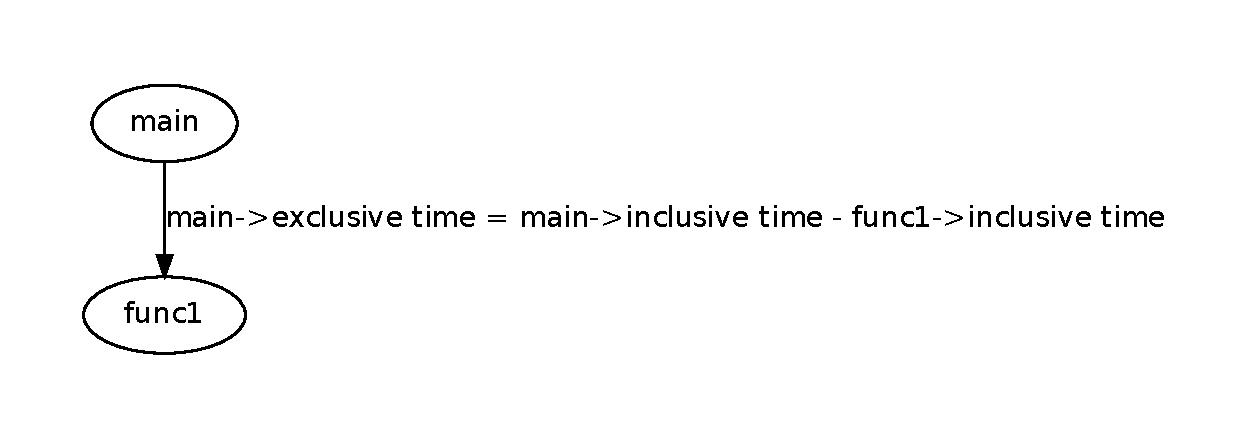
\includegraphics[scale=0.50]{images/tree2.pdf}
  \captionof{figure}{test2}
\end{center}

\begin{center}
  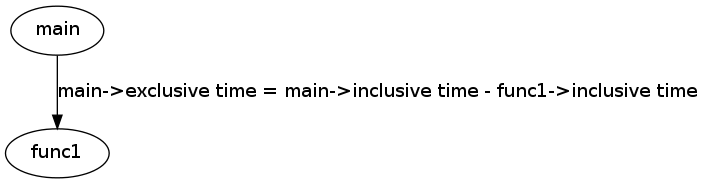
\includegraphics[scale=0.50]{images/tree.png}
  \captionof{figure}{test}
\end{center}
